\begin{frame}{\Naive{} Addressing Behaviour in Smart Environments}
  \centering
    \begin{columns}[T] % align columns
      \begin{column}{.5\textwidth}
        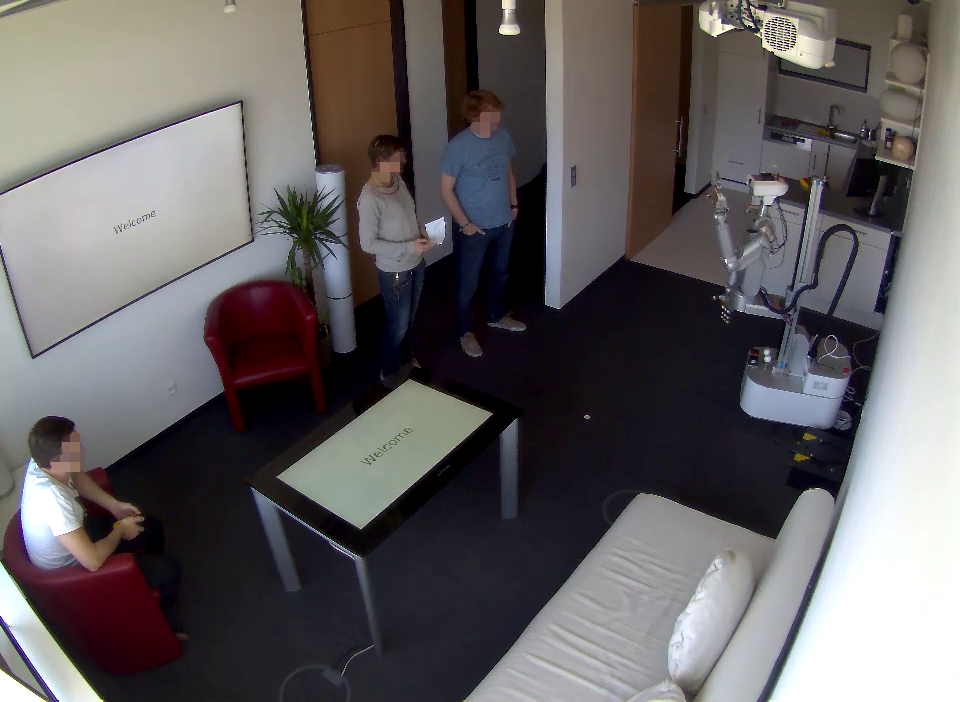
\includegraphics[trim={8cm 5cm 2cm 0cm},clip,width=\textwidth]{study-addressee-vp57-cam1}
      \end{column}
      \begin{column}{.5\textwidth}
        \vspace{40pt}
        \textbf{RQ1: Addressing Behaviour}\\\vspace{5pt} 
        \onslide<2->{In \textcolor{myblue}{\naive{}} human interaction with a smart environment: }\onslide<3->{Which \textcolor{myblue}{behaviours} can be observed}\onslide<4->{ to distinguish \textcolor{myblue}{addressed} entities?}
      \end{column}
    \end{columns}
    \pnote{40-33}
\end{frame}
\begin{frame}{Addressing Apartment Study}
  \begin{columns}[T] % align columns
    \begin{column}{.5\textwidth}
      \centering
      \vspace{-10pt}
      \resizebox{1.\textwidth}{!}{%
        \footnotesize
        \begin{tikzpicture}
          \action<1->{\node (a) at (0,0)
          {
            \resizebox{1.\textwidth}{!}{%
              \def\svgwidth{1.3\textwidth}
              \input{generated/csra_map_study_addressee.pdf_tex}
            }
          };}
        \end{tikzpicture}
      }
    \end{column}
    \begin{column}{.5\textwidth}
      \onslide<1->{Solve 7 Daily Tasks \\}
      \vspace{5pt}
      \onslide<2->{WoZ \(\rightarrow\) Any solution possible \\}
      \vspace{5pt}
      \onslide<3->{
        Participants: 47 (25w, 22m)\\
        {\scriptsize \(18 \leq \text{age} \leq 50\), \(\mu_{age}=25.26\), \(\sigma_{age}=5.69\)\\}
      \vspace{5pt}
      \onslide<4->{Study Aim\obcite{4-}{Bernotat2016}: Solutions \& Addressees \\}}
    \end{column}
  \end{columns}
  \centering
  \onslide<5->{
    \textcolor{mygreen}{\textbf{My Aim: Find out how participants address entities!}}\obcite{5-}{Richter2016}
  }
  \pnote{
    40-33 - use the apartment study we conducted in the csra
  }
\end{frame}
\begin{frame}{Observations of Addressing Behaviour}
  \onslide<1->{I extract properties of \textcolor{mygreen}{successfull communication attempts} from the corpus\obcite{1-}{Holthaus2016a}}
    \vspace{10pt}
    \\\onslide<2->{\textcolor{mypurple}{\textbf{Addressee}}}
    \\\onslide<3->{\textcolor{myorange}{\textbf{Speech}} \hspace{2pt} Naming, Politeness, Phrasing, Sentence, Keywords}
    \\\onslide<4->{\textcolor{myyellow!80!black}{\textbf{Visual}} \hspace{2pt} Attention, Modality, Gestures, Emotions, Participant}
    \\\onslide<5->{\textcolor{mygray}{\textbf{Other}} \hspace{2pt} Task Order, Condition, Wizard Addressee, Task, Addressee is Attention}
    \\\onslide<6->{\begin{center}\textcolor{mygreen}{\faArrowRight} \textbf{307} observations in \textbf{16} variables\end{center}}
  \pnote{
    40-33 - elan annotations at time of wizard action
  }
\end{frame}
\begin{frame}{Addressee Recognition Models}
  \begin{columns}[T] % align columns
    \begin{column}{.25\textwidth}
      \centering
      \vspace{5pt}
      Bayesian Networks:\\
      \onslide<2->{\textcolor{myred}{Attention}\\}
      \onslide<3->{\textcolor{myblue}{Manual}\\}
       \vspace{5pt}
       Variable Sets:\\
       \onslide<4->{Speech\\}
       \onslide<5->{Visual\\}
       \onslide<6->{Speech + Visual\\}
       \onslide<7->{All\\}
    \end{column}
    \hspace{-.05\textwidth}
    \begin{column}{.8\textwidth}
      \centering
      \begin{tikzpicture}
       \action<2->{\node (a) at (0,0)
       {
         \resizebox{.32\textwidth}{!}{%
           \def\svgwidth{.45\textwidth}
           \input{generated/bn-attention-defence.pdf_tex}
         }
       };}
       \action<3->{\node (a) at (0,-.25\textwidth)
       {
         \resizebox{.95\textwidth}{!}{%
           \def\svgwidth{1.2\textwidth}
           \input{generated/bn-manual-defence.pdf_tex}
         }
       };}
      \end{tikzpicture}
    \end{column}
  \end{columns}
  \pnote{
    40-33 - after investigating correlations btw. vars\\
    manual represents dependency structure as understood by an expert
  }
\end{frame}
\begin{frame}{Addressee Recognition Results}
  \begin{columns}[T] % align columns
    \begin{column}{.45\textwidth}
      \centering
      \resizebox{1.\textwidth}{!}{%
          %\Large
          \begin{tikzpicture}
          \action<1->{\node (a) at (0,0)
          {
            \resizebox{1.\textwidth}{!}{%
              % Created by tikzDevice version 0.12
% !TEX encoding = UTF-8 Unicode
\begin{tikzpicture}[x=1pt,y=1pt]
\definecolor{fillColor}{RGB}{255,255,255}
\path[use as bounding box,fill=fillColor,fill opacity=0.00] (0,0) rectangle (398.34,492.35);
\begin{scope}
\path[clip] (  0.00,  0.00) rectangle (398.34,492.35);
\definecolor{drawColor}{RGB}{255,255,255}
\definecolor{fillColor}{gray}{0.98}

\path[draw=drawColor,line width= 0.6pt,line join=round,line cap=round,fill=fillColor] (  0.00,  0.00) rectangle (398.34,492.35);
\end{scope}
\begin{scope}
\path[clip] ( 39.80, 44.70) rectangle (123.94,470.59);
\definecolor{fillColor}{gray}{0.92}

\path[fill=fillColor] ( 39.80, 44.70) rectangle (123.94,470.59);
\definecolor{drawColor}{RGB}{255,255,255}

\path[draw=drawColor,line width= 0.3pt,line join=round] ( 39.80,113.30) --
	(123.94,113.30);

\path[draw=drawColor,line width= 0.3pt,line join=round] ( 39.80,211.76) --
	(123.94,211.76);

\path[draw=drawColor,line width= 0.3pt,line join=round] ( 39.80,310.23) --
	(123.94,310.23);

\path[draw=drawColor,line width= 0.3pt,line join=round] ( 39.80,408.70) --
	(123.94,408.70);

\path[draw=drawColor,line width= 0.6pt,line join=round] ( 39.80, 64.06) --
	(123.94, 64.06);

\path[draw=drawColor,line width= 0.6pt,line join=round] ( 39.80,162.53) --
	(123.94,162.53);

\path[draw=drawColor,line width= 0.6pt,line join=round] ( 39.80,261.00) --
	(123.94,261.00);

\path[draw=drawColor,line width= 0.6pt,line join=round] ( 39.80,359.46) --
	(123.94,359.46);

\path[draw=drawColor,line width= 0.6pt,line join=round] ( 39.80,457.93) --
	(123.94,457.93);

\path[draw=drawColor,line width= 0.6pt,line join=round] ( 62.75, 44.70) --
	( 62.75,470.59);

\path[draw=drawColor,line width= 0.6pt,line join=round] (100.99, 44.70) --
	(100.99,470.59);
\definecolor{fillColor}{RGB}{228,26,28}

\path[fill=fillColor] ( 45.54, 64.06) rectangle ( 79.96,180.65);
\definecolor{fillColor}{RGB}{55,126,184}

\path[fill=fillColor] ( 83.78, 64.06) rectangle (118.20,279.51);
\definecolor{drawColor}{RGB}{0,0,0}

\path[draw=drawColor,line width= 0.6pt,line join=round] ( 58.93,201.13) --
	( 66.57,201.13);

\path[draw=drawColor,line width= 0.6pt,line join=round] ( 62.75,201.13) --
	( 62.75,160.56);

\path[draw=drawColor,line width= 0.6pt,line join=round] ( 58.93,160.56) --
	( 66.57,160.56);

\path[draw=drawColor,line width= 0.6pt,line join=round] ( 97.17,301.56) --
	(104.82,301.56);

\path[draw=drawColor,line width= 0.6pt,line join=round] (100.99,301.56) --
	(100.99,257.45);

\path[draw=drawColor,line width= 0.6pt,line join=round] ( 97.17,257.45) --
	(104.82,257.45);
\end{scope}
\begin{scope}
\path[clip] (129.44, 44.70) rectangle (213.57,470.59);
\definecolor{fillColor}{gray}{0.92}

\path[fill=fillColor] (129.44, 44.70) rectangle (213.57,470.59);
\definecolor{drawColor}{RGB}{255,255,255}

\path[draw=drawColor,line width= 0.3pt,line join=round] (129.44,113.30) --
	(213.57,113.30);

\path[draw=drawColor,line width= 0.3pt,line join=round] (129.44,211.76) --
	(213.57,211.76);

\path[draw=drawColor,line width= 0.3pt,line join=round] (129.44,310.23) --
	(213.57,310.23);

\path[draw=drawColor,line width= 0.3pt,line join=round] (129.44,408.70) --
	(213.57,408.70);

\path[draw=drawColor,line width= 0.6pt,line join=round] (129.44, 64.06) --
	(213.57, 64.06);

\path[draw=drawColor,line width= 0.6pt,line join=round] (129.44,162.53) --
	(213.57,162.53);

\path[draw=drawColor,line width= 0.6pt,line join=round] (129.44,261.00) --
	(213.57,261.00);

\path[draw=drawColor,line width= 0.6pt,line join=round] (129.44,359.46) --
	(213.57,359.46);

\path[draw=drawColor,line width= 0.6pt,line join=round] (129.44,457.93) --
	(213.57,457.93);

\path[draw=drawColor,line width= 0.6pt,line join=round] (152.38, 44.70) --
	(152.38,470.59);

\path[draw=drawColor,line width= 0.6pt,line join=round] (190.63, 44.70) --
	(190.63,470.59);
\definecolor{fillColor}{RGB}{228,26,28}

\path[fill=fillColor] (135.17, 64.06) rectangle (169.59,413.03);
\definecolor{fillColor}{RGB}{55,126,184}

\path[fill=fillColor] (173.42, 64.06) rectangle (207.84,409.09);
\definecolor{drawColor}{RGB}{0,0,0}

\path[draw=drawColor,line width= 0.6pt,line join=round] (148.56,427.21) --
	(156.21,427.21);

\path[draw=drawColor,line width= 0.6pt,line join=round] (152.38,427.21) --
	(152.38,398.85);

\path[draw=drawColor,line width= 0.6pt,line join=round] (148.56,398.85) --
	(156.21,398.85);

\path[draw=drawColor,line width= 0.6pt,line join=round] (186.80,423.66) --
	(194.45,423.66);

\path[draw=drawColor,line width= 0.6pt,line join=round] (190.63,423.66) --
	(190.63,394.52);

\path[draw=drawColor,line width= 0.6pt,line join=round] (186.80,394.52) --
	(194.45,394.52);
\end{scope}
\begin{scope}
\path[clip] (219.07, 44.70) rectangle (303.21,470.59);
\definecolor{fillColor}{gray}{0.92}

\path[fill=fillColor] (219.07, 44.70) rectangle (303.21,470.59);
\definecolor{drawColor}{RGB}{255,255,255}

\path[draw=drawColor,line width= 0.3pt,line join=round] (219.07,113.30) --
	(303.21,113.30);

\path[draw=drawColor,line width= 0.3pt,line join=round] (219.07,211.76) --
	(303.21,211.76);

\path[draw=drawColor,line width= 0.3pt,line join=round] (219.07,310.23) --
	(303.21,310.23);

\path[draw=drawColor,line width= 0.3pt,line join=round] (219.07,408.70) --
	(303.21,408.70);

\path[draw=drawColor,line width= 0.6pt,line join=round] (219.07, 64.06) --
	(303.21, 64.06);

\path[draw=drawColor,line width= 0.6pt,line join=round] (219.07,162.53) --
	(303.21,162.53);

\path[draw=drawColor,line width= 0.6pt,line join=round] (219.07,261.00) --
	(303.21,261.00);

\path[draw=drawColor,line width= 0.6pt,line join=round] (219.07,359.46) --
	(303.21,359.46);

\path[draw=drawColor,line width= 0.6pt,line join=round] (219.07,457.93) --
	(303.21,457.93);

\path[draw=drawColor,line width= 0.6pt,line join=round] (242.02, 44.70) --
	(242.02,470.59);

\path[draw=drawColor,line width= 0.6pt,line join=round] (280.26, 44.70) --
	(280.26,470.59);
\definecolor{fillColor}{RGB}{228,26,28}

\path[fill=fillColor] (224.81, 64.06) rectangle (259.23,413.03);
\definecolor{fillColor}{RGB}{55,126,184}

\path[fill=fillColor] (263.05, 64.06) rectangle (297.47,405.15);
\definecolor{drawColor}{RGB}{0,0,0}

\path[draw=drawColor,line width= 0.6pt,line join=round] (238.19,427.21) --
	(245.84,427.21);

\path[draw=drawColor,line width= 0.6pt,line join=round] (242.02,427.21) --
	(242.02,398.85);

\path[draw=drawColor,line width= 0.6pt,line join=round] (238.19,398.85) --
	(245.84,398.85);

\path[draw=drawColor,line width= 0.6pt,line join=round] (276.44,420.51) --
	(284.08,420.51);

\path[draw=drawColor,line width= 0.6pt,line join=round] (280.26,420.51) --
	(280.26,390.18);

\path[draw=drawColor,line width= 0.6pt,line join=round] (276.44,390.18) --
	(284.08,390.18);
\end{scope}
\begin{scope}
\path[clip] (308.71, 44.70) rectangle (392.84,470.59);
\definecolor{fillColor}{gray}{0.92}

\path[fill=fillColor] (308.71, 44.70) rectangle (392.84,470.59);
\definecolor{drawColor}{RGB}{255,255,255}

\path[draw=drawColor,line width= 0.3pt,line join=round] (308.71,113.30) --
	(392.84,113.30);

\path[draw=drawColor,line width= 0.3pt,line join=round] (308.71,211.76) --
	(392.84,211.76);

\path[draw=drawColor,line width= 0.3pt,line join=round] (308.71,310.23) --
	(392.84,310.23);

\path[draw=drawColor,line width= 0.3pt,line join=round] (308.71,408.70) --
	(392.84,408.70);

\path[draw=drawColor,line width= 0.6pt,line join=round] (308.71, 64.06) --
	(392.84, 64.06);

\path[draw=drawColor,line width= 0.6pt,line join=round] (308.71,162.53) --
	(392.84,162.53);

\path[draw=drawColor,line width= 0.6pt,line join=round] (308.71,261.00) --
	(392.84,261.00);

\path[draw=drawColor,line width= 0.6pt,line join=round] (308.71,359.46) --
	(392.84,359.46);

\path[draw=drawColor,line width= 0.6pt,line join=round] (308.71,457.93) --
	(392.84,457.93);

\path[draw=drawColor,line width= 0.6pt,line join=round] (331.65, 44.70) --
	(331.65,470.59);

\path[draw=drawColor,line width= 0.6pt,line join=round] (369.89, 44.70) --
	(369.89,470.59);
\definecolor{fillColor}{RGB}{228,26,28}

\path[fill=fillColor] (314.44, 64.06) rectangle (348.86,413.03);
\definecolor{fillColor}{RGB}{55,126,184}

\path[fill=fillColor] (352.68, 64.06) rectangle (387.10,442.57);
\definecolor{drawColor}{RGB}{0,0,0}

\path[draw=drawColor,line width= 0.6pt,line join=round] (327.83,427.21) --
	(335.47,427.21);

\path[draw=drawColor,line width= 0.6pt,line join=round] (331.65,427.21) --
	(331.65,398.85);

\path[draw=drawColor,line width= 0.6pt,line join=round] (327.83,398.85) --
	(335.47,398.85);

\path[draw=drawColor,line width= 0.6pt,line join=round] (366.07,451.23) --
	(373.72,451.23);

\path[draw=drawColor,line width= 0.6pt,line join=round] (369.89,451.23) --
	(369.89,433.90);

\path[draw=drawColor,line width= 0.6pt,line join=round] (366.07,433.90) --
	(373.72,433.90);
\end{scope}
\begin{scope}
\path[clip] ( 39.80,470.59) rectangle (123.94,486.85);
\definecolor{fillColor}{gray}{0.85}

\path[fill=fillColor] ( 39.80,470.59) rectangle (123.94,486.85);
\definecolor{drawColor}{gray}{0.10}

\node[text=drawColor,anchor=base,inner sep=0pt, outer sep=0pt, scale=  0.80] at ( 81.87,475.96) {Speech};
\end{scope}
\begin{scope}
\path[clip] (129.44,470.59) rectangle (213.57,486.85);
\definecolor{fillColor}{gray}{0.85}

\path[fill=fillColor] (129.44,470.59) rectangle (213.57,486.85);
\definecolor{drawColor}{gray}{0.10}

\node[text=drawColor,anchor=base,inner sep=0pt, outer sep=0pt, scale=  0.80] at (171.50,475.96) {Visual};
\end{scope}
\begin{scope}
\path[clip] (219.07,470.59) rectangle (303.21,486.85);
\definecolor{fillColor}{gray}{0.85}

\path[fill=fillColor] (219.07,470.59) rectangle (303.21,486.85);
\definecolor{drawColor}{gray}{0.10}

\node[text=drawColor,anchor=base,inner sep=0pt, outer sep=0pt, scale=  0.80] at (261.14,475.96) {Speech + Visual};
\end{scope}
\begin{scope}
\path[clip] (308.71,470.59) rectangle (392.84,486.85);
\definecolor{fillColor}{gray}{0.85}

\path[fill=fillColor] (308.71,470.59) rectangle (392.84,486.85);
\definecolor{drawColor}{gray}{0.10}

\node[text=drawColor,anchor=base,inner sep=0pt, outer sep=0pt, scale=  0.80] at (350.77,475.96) {All};
\end{scope}
\begin{scope}
\path[clip] (  0.00,  0.00) rectangle (398.34,492.35);
\definecolor{drawColor}{RGB}{0,0,0}

\node[text=drawColor,anchor=base east,inner sep=0pt, outer sep=0pt, scale=  1.00] at ( 34.85, 60.62) {0.00};

\node[text=drawColor,anchor=base east,inner sep=0pt, outer sep=0pt, scale=  1.00] at ( 34.85,159.09) {0.25};

\node[text=drawColor,anchor=base east,inner sep=0pt, outer sep=0pt, scale=  1.00] at ( 34.85,257.55) {0.50};

\node[text=drawColor,anchor=base east,inner sep=0pt, outer sep=0pt, scale=  1.00] at ( 34.85,356.02) {0.75};

\node[text=drawColor,anchor=base east,inner sep=0pt, outer sep=0pt, scale=  1.00] at ( 34.85,454.49) {1.00};
\end{scope}
\begin{scope}
\path[clip] (  0.00,  0.00) rectangle (398.34,492.35);
\definecolor{drawColor}{RGB}{0,0,0}

\node[text=drawColor,rotate= 90.00,anchor=base,inner sep=0pt, outer sep=0pt, scale=  1.00] at ( 12.39,257.65) {Accuracy with 95\% confidence intervals};
\end{scope}
\begin{scope}
\path[clip] (  0.00,  0.00) rectangle (398.34,492.35);
\definecolor{fillColor}{RGB}{255,255,255}

\path[fill=fillColor] (127.88,  5.50) rectangle (304.77, 30.95);
\end{scope}
\begin{scope}
\path[clip] (  0.00,  0.00) rectangle (398.34,492.35);
\definecolor{drawColor}{RGB}{0,0,0}

\node[text=drawColor,anchor=base west,inner sep=0pt, outer sep=0pt, scale=  1.00] at (133.38, 14.78) {Model};
\end{scope}
\begin{scope}
\path[clip] (  0.00,  0.00) rectangle (398.34,492.35);
\definecolor{drawColor}{RGB}{255,255,255}
\definecolor{fillColor}{gray}{0.95}

\path[draw=drawColor,line width= 0.6pt,line join=round,line cap=round,fill=fillColor] (175.59, 11.00) rectangle (190.05, 25.45);
\end{scope}
\begin{scope}
\path[clip] (  0.00,  0.00) rectangle (398.34,492.35);
\definecolor{fillColor}{RGB}{228,26,28}

\path[fill=fillColor] (176.31, 11.71) rectangle (189.34, 24.74);
\end{scope}
\begin{scope}
\path[clip] (  0.00,  0.00) rectangle (398.34,492.35);
\definecolor{drawColor}{RGB}{255,255,255}
\definecolor{fillColor}{gray}{0.95}

\path[draw=drawColor,line width= 0.6pt,line join=round,line cap=round,fill=fillColor] (243.60, 11.00) rectangle (258.05, 25.45);
\end{scope}
\begin{scope}
\path[clip] (  0.00,  0.00) rectangle (398.34,492.35);
\definecolor{fillColor}{RGB}{55,126,184}

\path[fill=fillColor] (244.31, 11.71) rectangle (257.34, 24.74);
\end{scope}
\begin{scope}
\path[clip] (  0.00,  0.00) rectangle (398.34,492.35);
\definecolor{drawColor}{RGB}{0,0,0}

\node[text=drawColor,anchor=base west,inner sep=0pt, outer sep=0pt, scale=  0.80] at (195.05, 15.47) {Attention};
\end{scope}
\begin{scope}
\path[clip] (  0.00,  0.00) rectangle (398.34,492.35);
\definecolor{drawColor}{RGB}{0,0,0}

\node[text=drawColor,anchor=base west,inner sep=0pt, outer sep=0pt, scale=  0.80] at (263.05, 15.47) {Manual};
\end{scope}
\end{tikzpicture}

            }
          };}
          \action<1>{\filldraw [fill=bgcolorframe, draw=bgcolorframe] (3.3,3.5) rectangle (-2.5,-3.2);}
          \action<2>{\filldraw [fill=bgcolorframe, draw=bgcolorframe] (3.3,3.5) rectangle (-1.1,-3.2);}
          \action<3>{\filldraw [fill=bgcolorframe, draw=bgcolorframe] (3.3,3.5) rectangle (0.2,-3.2);}
          \action<4>{\filldraw [fill=bgcolorframe, draw=bgcolorframe] (3.3,3.5) rectangle (1.6,-3.2);}
         \end{tikzpicture}
       }
    \end{column}
    \hspace{20pt}
    \begin{column}{.55\textwidth}
      \resizebox{1.2\textwidth}{!}{%
      \begin{tikzpicture}
        \hspace{-40pt}
         \node (a) at (0,0)
         {
           \resizebox{.32\textwidth}{!}{%
             \def\svgwidth{.9\textwidth}
             \input{generated/bn-attention-defence.pdf_tex}
           }
         };
         \node (a) at (.6\textwidth,0)
         {
           \resizebox{.8\textwidth}{!}{%
             \def\svgwidth{2.2\textwidth}
             \input{generated/bn-manual-defence.pdf_tex}
           }
         };
        \end{tikzpicture}
      }
      \vspace{0pt}
      \footnotesize
      \begin{itemize}
        \item[\textbf{Speech}] \action<2->{\(Attention\) has no Information\\\(Manual\) predicts \(\approx 55\%\)}
        \item[\textbf{Visual}] \action<3->{Both around \(89\%\), \\\(Attention\) cannot be outperformed} 
        \item[\textbf{Speech+Visual}] \action<4->{\(Attention\) cannot be outperformed}
        \item[\textbf{All}] \action<5->{\(Manual\) achieves \(\approx 96\%\)}
      \end{itemize}
    \end{column}
  \end{columns}
  \pnote{
    40-33
  }
\end{frame}
\begin{frame}{Summary RQ1}
  I Investigated:\\
  \begin{itemize}
    \item<1->[\textcolor{mygreen}{\faCheckCircle}] \textcolor{myblue}{Addressing behaviour} of \textcolor{myblue}{\naive{}} users in a smart environment. 
    \item<2->[\textcolor{mygreen}{\faCheckCircle}] \textcolor{myblue}{Attention} is the most important information in addressing (\(\approx 89\%\)).
    \item<3->[\textcolor{mygreen}{\faCheckCircle}] \textcolor{myblue}{Speech} can predict addressee in \(\approx 55\%\) of interactions.
  \end{itemize}
  \pnote{40-33}
\end{frame}
\begin{frame}{Overview}
    \emph{\goalshort}
    \centering\\
    \vspace{10pt}
    \resizebox{1.\textwidth}{!}{%
        \footnotesize
        \begin{tikzpicture}
        \action<1->{\node (a) at (0,0)
        {
          \resizebox{.25\textwidth}{!}{%
            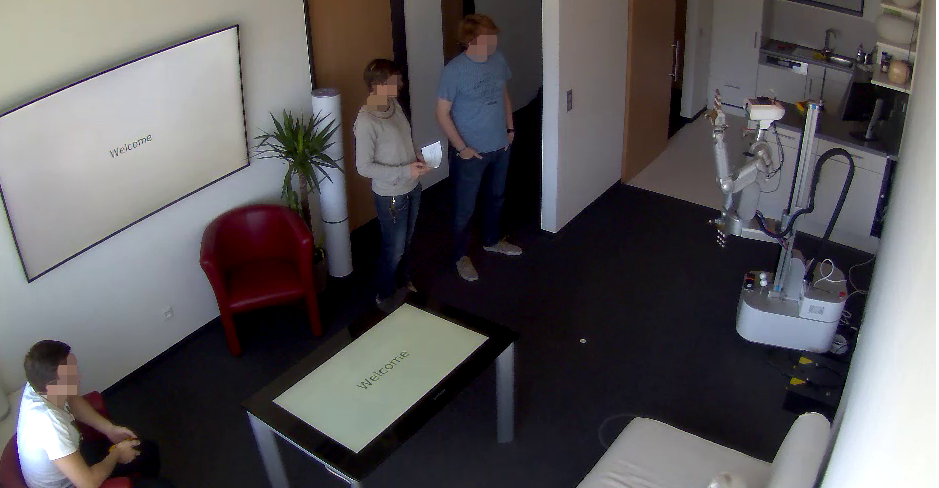
\includegraphics[trim={8cm 0 2cm 0},clip]{study-addressee-vp57}
          }
        };}
        \action<1->{\node[align=left, anchor=north, text width=.25\textwidth] (at) at (0, -.11\textwidth) {
        \textbf{RQ1 \scriptsize Addressing Behaviour}\\
          \vspace{5pt}
          \textcolor{mygreen}{\faCheckCircle} \Naive{} addressing\\
          \textcolor{mygreen}{\faCheckCircle} Attention\\
          \textcolor{mygreen}{\faCheckCircle} Speech
        };}
        \action<1->{\node (b) at (.25\textwidth+10,0)
        {
          \resizebox{.25\textwidth}{!}{%
            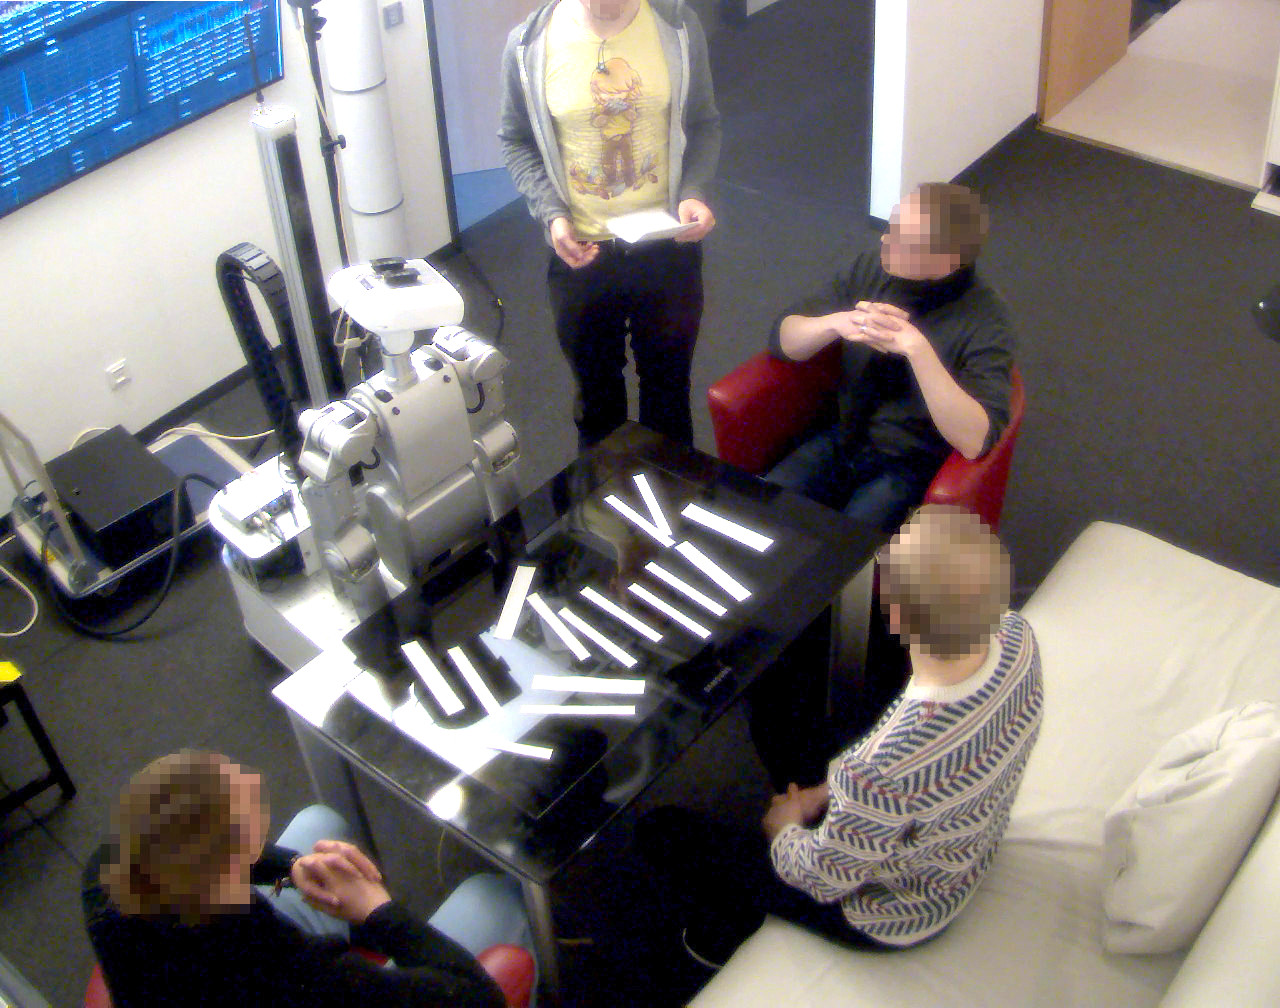
\includegraphics[trim={0 0 0 2cm},clip]{addressee-meka-intro}
          }
        };}
        \action<1->{\node[align=center, anchor=north, text width=.25\textwidth] (bt) at (.25\textwidth+10, -.11\textwidth) {
          \textbf{RQ2 \scriptsize Addressee Recognition}\\
          \vspace{5pt}
          React \\ to Addressing
          };}
        \action<1->{\node (c) at (.5\textwidth+20,0)
        {
          \resizebox{.25\textwidth}{!}{%
            \input{generated/conversational_group_defence.pdf_tex}
          }
        };}
        \action<1->{\node[align=center, anchor=north, text width=.25\textwidth] (ct) at (.5\textwidth+20, -.11\textwidth) {
          \textbf{RQ3 \scriptsize Conversational Group}\\
          \vspace{5pt}
          Participate \\ in Interaction
          };}
        \action<1->{\node (d) at (.75\textwidth+30,0)
        {
          \resizebox{.25\textwidth}{!}{%
            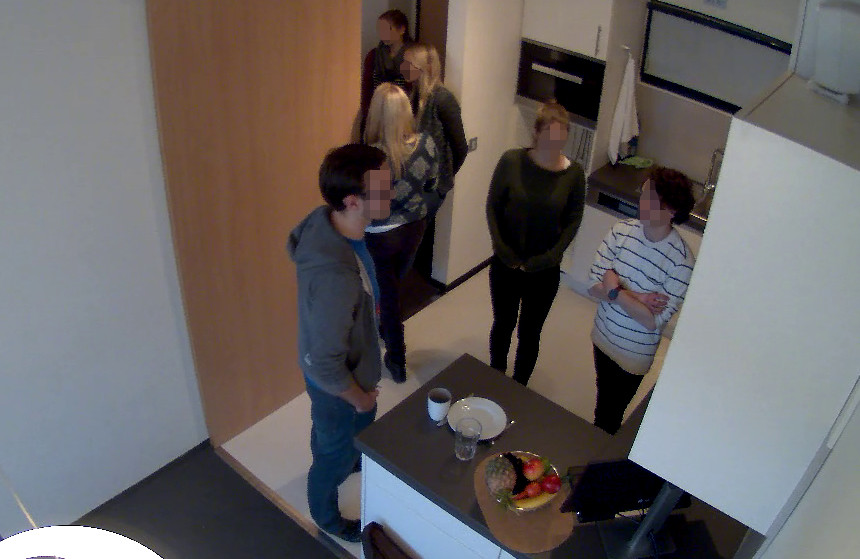
\includegraphics[trim={4.1cm 0 0 0},clip]{conversational_group}
          }
        };}
        \action<1->{\node[align=center, anchor=north, text width=.25\textwidth] (dt) at (.75\textwidth+30, -.11\textwidth) {
          \textbf{RQ4 \scriptsize Conversational Roles}\\
          \vspace{5pt}
          Repair \\ Interaction
        };}
        \action<1>{\filldraw [fill=bgcolorframe, draw=bgcolorframe, opacity=0.8, fill opacity=0.8] (380pt,-150pt) rectangle (50pt,40pt);}
        \action<2>{\filldraw [fill=bgcolorframe, draw=bgcolorframe, opacity=0.8, fill opacity=0.8] (380pt,-150pt) rectangle (160pt,40pt);}
\end{tikzpicture}
      }
\end{frame}
